% Three tokenizer modes side by side -- companion slide to tokenizer.tex.
% Compile: pdflatex modes.tex  (standalone class, standard TikZ only)
\documentclass[tikz,border=8pt]{standalone}
\usepackage{amsmath,amssymb}
\usetikzlibrary{positioning,arrows.meta,calc}

\definecolor{rawc}{RGB}{56,108,176}
\definecolor{pacc}{RGB}{217,120,44}
\definecolor{annot}{RGB}{105,105,105}

\tikzset{
  lbl/.style={font=\small\bfseries, align=center},
  note/.style={font=\scriptsize, text=annot, align=center},
  win/.style={font=\scriptsize, align=center},
}

% #1 = origin coordinate name (top-left of block), #2 = fill color
% draws 4 rows x 5 cols of 3.0mm cells on a 3.2mm pitch, growing downward
\newcommand{\gridblock}[2]{%
  \foreach \r in {0,1,2,3} {
    \foreach \c in {0,1,2,3,4} {
      \fill[#2!25, draw=#2!60, line width=0.3pt]
        ($(#1)+(\c*3.2mm,-\r*3.2mm)$) rectangle ++(3.0mm,-3.0mm);
    }
  }
}

\begin{document}
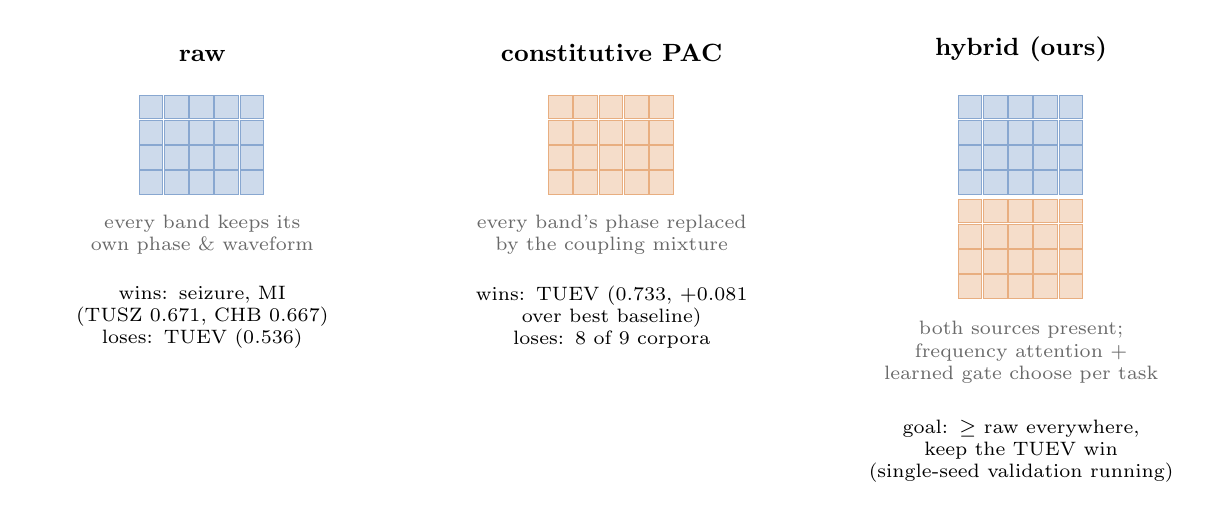
\begin{tikzpicture}

% ------------------------------------------------- (a) raw
\coordinate (A) at (0,0);
\node[lbl, anchor=south] at ($(A)+(8mm,3mm)$) {raw};
\gridblock{A}{rawc}
\node[note, anchor=north, text width=40mm] at ($(A)+(8mm,-14mm)$)
  {every band keeps its\\ own phase \& waveform};
\node[win, anchor=north, text width=42mm] at ($(A)+(8mm,-23mm)$)
  {wins: seizure, MI\\ {\scriptsize (TUSZ $0.671$, CHB $0.667$)}\\
   loses: TUEV ($0.536$)};

% ------------------------------------------------- (b) constitutive PAC
\coordinate (B) at (5.2,0);
\node[lbl, anchor=south] at ($(B)+(8mm,3mm)$) {constitutive PAC};
\gridblock{B}{pacc}
\node[note, anchor=north, text width=40mm] at ($(B)+(8mm,-14mm)$)
  {every band's phase replaced\\ by the coupling mixture};
\node[win, anchor=north, text width=42mm] at ($(B)+(8mm,-23mm)$)
  {wins: TUEV ($0.733$, $+0.081$\\ over best baseline)\\
   loses: 8 of 9 corpora};

% ------------------------------------------------- (c) hybrid
\coordinate (C) at (10.4,0);
\coordinate (Clow) at ($(C)+(0,-13.2mm)$);
\node[lbl, anchor=south] at ($(C)+(8mm,3mm)$) {hybrid (ours)};
\gridblock{C}{rawc}
\gridblock{Clow}{pacc}
\node[note, anchor=north, text width=42mm] at ($(C)+(8mm,-27.5mm)$)
  {both sources present;\\ frequency attention +\\ learned gate choose per task};
\node[win, anchor=north, text width=42mm] at ($(C)+(8mm,-40mm)$)
  {goal: $\geq$ raw everywhere,\\ keep the TUEV win\\
   {\scriptsize (single-seed validation running)}};

\end{tikzpicture}
\end{document}
